\documentclass[11pt,a4paper]{article}
\usepackage[utf8]{inputenc}
\usepackage[margin=1in]{geometry}
\usepackage{tabularx}
\usepackage{booktabs}
\usepackage{hyperref}
\usepackage{graphicx}
\usepackage{lmodern}
\usepackage{float}
\usepackage{tikz}
\usepackage{microtype}
\usepackage[table]{xcolor}
\usetikzlibrary{arrows.meta,positioning,shapes.geometric,fit,calc}

\setlength{\parindent}{0pt}
\setlength{\parskip}{0.6em}
\renewcommand{\arraystretch}{1.2}

\newcolumntype{L}[1]{>{\raggedright\arraybackslash}p{#1}}
\newcolumntype{Y}{>{\raggedright\arraybackslash}X}

\newcommand{\screenshotorplaceholder}[2]{%
\IfFileExists{#1}{%
\includegraphics[width=\linewidth]{#1}%
}{%
\fbox{\parbox[c][0.24\textheight][c]{0.95\linewidth}{\centering
Screenshot placeholder\\[0.5em]
\texttt{\detokenize{#1}}\\[0.4em]
#2
}}
}%
}

\title{GraphRAG Implementation Plan \\ \large Product Information \& Compatibility: Building Automation \& HVAC Controls} 

\author{%
    \begin{tabular}[t]{ccc}
        Varad Paradkar & Nidhi Shah & Brinda Chinnaraji \\[0.3em]
        \multicolumn{3}{c}{Sai Kiran Jagini \quad Shar Adhiambo}
    \end{tabular}%
}

\date{\today}

\begin{document}

\maketitle

\tableofcontents
\newpage

\section{Introduction}
This document outlines a first-draft plan for implementing a GraphRAG (Graph Retrieval-Augmented Generation) pipeline for querying product compatibility information in Building Automation and HVAC systems. The pipeline covers five stages, graph construction, query understanding, graph traversal, context assembly, and LLM generation, and is grounded in the Honeywell Home T9 Wi-Fi Thermostat Installation Guide as the source document.

\section{Source Document, Data References \& Domain Justification}
This section identifies what data is in the source document, where specifically that data is located, and why it is appropriate for the stated domain of Building Automation and HVAC Controls.

\subsection{Source Document: Honeywell Home T9 Wi-Fi Thermostat Installation Guide}
This is the official installation guide for the Honeywell Home T9 smart thermostat, a Wi-Fi connected HVAC controller with wireless room sensor support, geofencing, and motion-based room prioritisation. It defines system compatibility, wiring terminals, electrical requirements, and accessory relationships that are directly relevant to HVAC graph modelling.

The table below maps each piece of data referenced in this report to its exact location in the document:

\begin{table}[H]
\centering
\small
\setlength{\tabcolsep}{6pt}
\rowcolors{2}{gray!8}{white}
\begin{tabularx}{\textwidth}{L{0.52\textwidth}Y}
\toprule
\rowcolor{gray!18}
\textbf{Data Referenced in Report} & \textbf{Exact Location in Document} \\
\midrule
Thermostat model: T9 Wi-Fi Thermostat & Page 1 title and cover page \\
Electrical specification: 24V AC, 60Hz, 0.2A input & Page 3 -- Electrical Specifications section \\
C-Wire requirement: required for 24 VAC power; C-Wire Adapter included if absent & Page 3 -- Electrical Specifications section \\
Compatible systems: most heating, cooling, and heat pump systems & Page 3 -- Compatibility section (bullet point 1) \\
Incompatible systems: electric baseboard heat (120--240V), millivolt systems & Page 3 -- Compatibility section (bullet points 2 and 3) \\
Does not support S terminals for indoor/outdoor sensors & Page 3 -- Compatibility section (bullet point 4) \\
Wiring terminals: C, Y, G, R, Rc, Rh, W, W2/Aux, O/B, E, K, $U(1/2)$, A, Y2 & Page 6 -- Step 8 wire checklist table \\
Accessory: Wireless Room Sensor, up to 20 sensors and up to 200-foot range & Page 13 -- Whole-Home Range feature description \\
Sensor capabilities: temperature, humidity, and occupancy (motion) detection & Page 13 -- Whole-Home Range feature description \\
Room priority modes: Selected Rooms and Active Rooms (motion-based) & Page 15 -- Using Priority section \\
Troubleshooting temperature ranges: Heat $40$--$90^{\circ}F$, Cool $50$--$99^{\circ}F$ & Page 16 -- Troubleshooting table \\
Smartphone requirement: Android or iOS device & Page 3 -- Compatibility section \\
Zoning panel caveat: C-Wire Adapter install is more complex on zoned systems & Page 7 -- Step 11 compatibility check \\
Warranty: 2-year limited warranty by Resideo & Page 17 -- 2-year limited warranty section \\
\bottomrule
\end{tabularx}
\caption{Traceability mapping between referenced HVAC facts and source-page evidence.}
\label{tab:source-traceability}
\end{table}

\subsection{Domain Fit Assessment}
The domain for this project is Building Automation and HVAC Controls. The T9 Installation Guide is a strong and direct fit for this domain:

\textbf{Why the T9 Thermostat Installation Guide is appropriate:}
The T9 is a genuine HVAC device. The installation guide defines typed compatibility relationships (compatible vs. not compatible system types), wiring terminal connections (C, Y, G, R, W, O/B, and others), accessory pairings (room sensors with quantity and range limits), and electrical constraints (24V AC, C-wire requirement). These are exactly the kind of structured, typed relationships that map naturally onto a knowledge graph with quantitative edge properties.

Real-world HVAC compatibility questions, `Is the T9 compatible with my heat pump?', `Do I need a C-Wire Adapter?', `How many room sensors can I add?', `What wiring terminals does it use?', are all directly answerable from the graph built from this document.

\subsection{Why This Document Is Suited to Graph Construction and Querying}

\begin{table}[H]
\centering
\small
\setlength{\tabcolsep}{6pt}
\rowcolors{2}{gray!8}{white}
\begin{tabularx}{\textwidth}{L{0.30\textwidth}Y}
\toprule
\rowcolor{gray!18}
\textbf{Graph Requirement} & \textbf{How the T9 Document Meets It} \\
\midrule
Typed nodes (entities) & Thermostat, HVAC system type, wiring terminal, room sensor, C-Wire Adapter, and zoning panel are all clearly defined with distinct identifiers and attributes. \\
Typed edges (relationships) & COMPATIBLE\_WITH (system types), NOT\_COMPATIBLE\_WITH (excluded systems with reasons), REQUIRES (wiring terminals), CONNECTS\_TO (room sensors), NEEDS\_ADAPTER\_IF\_MISSING (C-Wire Adapter condition). \\
Edge properties for filtering & max\_sensors $=20$, sensor\_range\_ft $=200$, voltage $=24V$ AC, terminal labels, sensor\_capabilities = [temperature, humidity, occupancy]. \\
Real-world query value & Installers and homeowners ask compatibility questions that are directly answerable from this graph: system type fit, wiring needs, accessory limits, and operating constraints. \\
Multi-hop traversal potential & Example: T9 Thermostat $\rightarrow$ CONNECTS\_TO Room Sensor $\rightarrow$ capabilities. Or: T9 $\rightarrow$ NOT\_COMPATIBLE\_WITH Electric Baseboard $\rightarrow$ reason (line voltage 120--240V). \\
Scalability & The T9 node and relationships provide a reusable template for adding additional thermostat models without changing schema design. \\
\bottomrule
\end{tabularx}
\caption{Why the T9 installation guide is well-suited for graph construction and GraphRAG querying.}
\label{tab:graph-fit}
\end{table}

\section{Pipeline Overview}
The GraphRAG pipeline consists of five stages, each described in the following sections.

\begin{description}
    \item[Stage 1: Graph Construction] Extract entities and relationships from the T9 Installation Guide and load them into a graph database.
    \item[Stage 2: Query Understanding] Parse a user's natural language question to identify what entities and relationships are being asked about.
    \item[Stage 3: Graph Traversal] Search the graph to find the nodes and edges that answer the query.
    \item[Stage 4: Context Assembly] Collect the retrieved graph results into a structured context block.
    \item[Stage 5: LLM Generation] Pass the context to a language model to produce a clear, grounded natural language response.
\end{description}

\subsection{TikZ Architecture Diagram}
Figure~\ref{fig:tikz-architecture} shows the Week 1 reference architecture for the implementation.

\begin{figure}[H]
\centering
\makebox[\textwidth][c]{%
\resizebox{0.95\textwidth}{!}{%
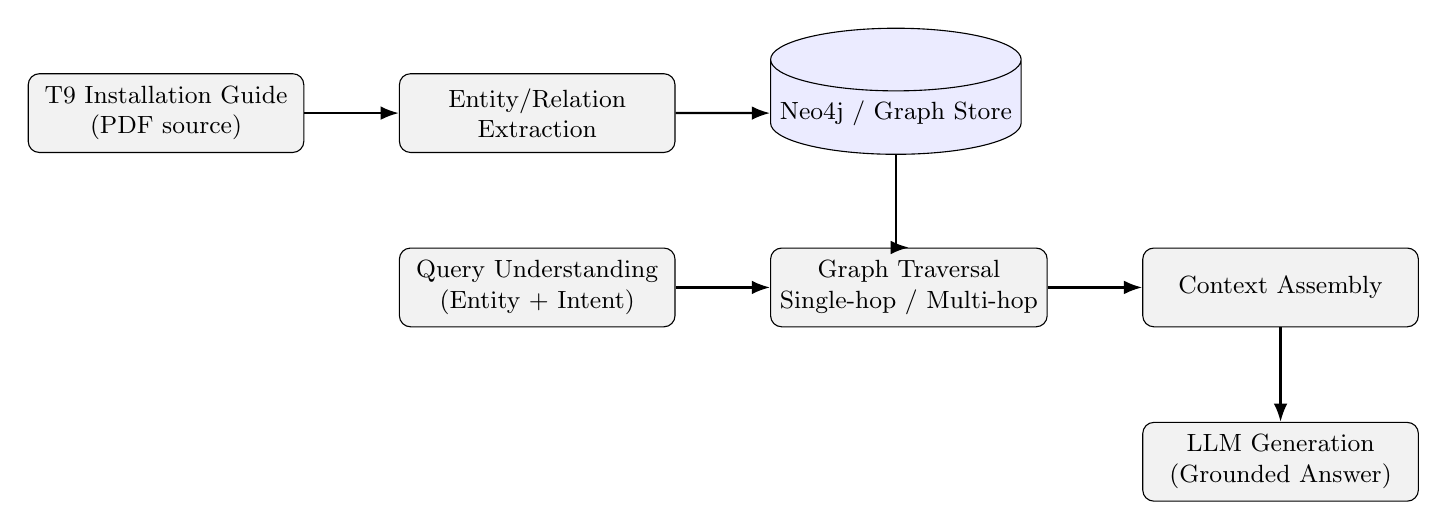
\begin{tikzpicture}[
    font=\small,
    node distance=0.9cm and 1.2cm,
    block/.style={draw, rounded corners, align=center, minimum width=3.5cm, minimum height=1.0cm, fill=gray!10},
    db/.style={draw, cylinder, shape border rotate=90, aspect=0.25, align=center, minimum height=1.3cm, minimum width=2.8cm, fill=blue!8},
    line/.style={-Latex, thick}
]
    \node[block] (pdf) {T9 Installation Guide\\(PDF source)};
    \node[block, right=of pdf] (extract) {Entity/Relation\\Extraction};
    \node[db, right=of extract] (graphdb) {Neo4j / Graph Store};

    \node[block, below=1.2cm of extract] (query) {Query Understanding\\(Entity + Intent)};
    \node[block, right=of query] (traverse) {Graph Traversal\\Single-hop / Multi-hop};
    \node[block, right=of traverse] (context) {Context Assembly};
    \node[block, below=1.2cm of context] (llm) {LLM Generation\\(Grounded Answer)};

    \draw[line] (pdf) -- (extract);
    \draw[line] (extract) -- (graphdb);
    \draw[line] (query) -- (traverse);
    \draw[line] (traverse) -- (context);
    \draw[line] (context) -- (llm);
    \draw[line] (graphdb.south) |- (traverse.north);
\end{tikzpicture}
}}
\caption{GraphRAG pipeline architecture for Deliverable 1 (Week 1 baseline).}
\label{fig:tikz-architecture}
\end{figure}

\section{Stage 1: Graph Construction}
The first stage builds the knowledge graph from the T9 Installation Guide. Entities become nodes and their relationships become edges. Attribute values such as sensor limits, voltage requirements, and wiring terminal labels are stored as node or edge properties to enable precise filtering during traversal.

\textbf{Nodes (Entities)}
\begin{itemize}
    \item \textbf{Thermostat} - Honeywell Home T9 Wi-Fi Thermostat
    \item \textbf{HVAC System Type} - Heat Pump, Forced Air Heating, Central Cooling, Electric Baseboard (incompatible), Millivolt System (incompatible)
    \item \textbf{Wiring Terminal} - C, Y, G, R, Rc, Rh, W, W2/Aux, O/B, Y2, E, K, U
    \item \textbf{Room Sensor} - Wireless Room Sensor (accessory)
    \item \textbf{Adapter} - C-Wire Adapter (included accessory)
    \item \textbf{Zoning Panel} - multi-thermostat / single-furnace zoned system
\end{itemize}

\textbf{Relationships (Edges), with Properties}
\begin{itemize}
    \item \textbf{COMPATIBLE\_WITH} - Thermostat to HVAC System Type. Property: status = 'compatible'. Source: Page 3.
    \item \textbf{NOT\_COMPATIBLE\_WITH} - Thermostat to HVAC System Type. Property: reason (e.g., 'line voltage 120-240V', 'millivolt system'). Source: Page 3.
    \item \textbf{REQUIRES} - Thermostat to Wiring Terminal. Property: required = true/false. C-wire is required; others depend on system type. Source: Pages 3 and 6.
    \item \textbf{CONNECTS\_TO} - Thermostat to Room Sensor. Properties: max\_sensors $=20$, max\_range\_ft $=200$, capabilities = [temperature, humidity, occupancy]. Source: Page 13.
    \item \textbf{NEEDS\_ADAPTER\_IF\_MISSING} - Thermostat to C-Wire Adapter. Condition: triggered when no C-wire is present. Source: Pages 3 and 7.
    \item \textbf{COMPLEX\_ON} - C-Wire Adapter to Zoning Panel. Property: note = 'professional installer recommended'. Source: Page 7.
\end{itemize}

\textbf{Tools}
\begin{itemize}
    \item Graph database: Neo4j
    \item Query language: Cypher
    \item Data extraction: Python (pdfplumber / pandas) to parse content from the source PDF
\end{itemize}

\section{Stage 2: Query Understanding}
When a user asks a question in plain English, the system identifies three things before querying the graph: the subject entity, the relationship type being asked about, and any filters or constraints.

Examples from the T9 domain:
\begin{itemize}
    \item "Is the T9 compatible with my heat pump?" $\rightarrow$ Subject: T9 Thermostat, Relationship: COMPATIBLE\_WITH, Filter: system\_type = 'Heat Pump'
    \item "Do I need a C-Wire Adapter for the T9?" $\rightarrow$ Subject: T9 Thermostat, Relationship: REQUIRES + NEEDS\_ADAPTER\_IF\_MISSING, Return: C-wire requirement and adapter condition
    \item "How many room sensors can I add to the T9?" $\rightarrow$ Subject: T9 Thermostat, Relationship: CONNECTS\_TO, Return: max\_sensors property
    \item "What systems is the T9 not compatible with?" $\rightarrow$ Subject: T9 Thermostat, Relationship: NOT\_COMPATIBLE\_WITH, Return: all excluded system types with reasons
    \item "What wiring terminals does the T9 use?" $\rightarrow$ Subject: T9 Thermostat, Relationship: REQUIRES, Return: all connected Wiring Terminal nodes
\end{itemize}

An LLM or lightweight NLP layer handles this parsing and translates the result into a Cypher query ready for graph traversal.

\section{Stage 3: Graph Traversal}
With the query translated, the system traverses the graph to retrieve the relevant nodes and edges.

\textbf{Single-Hop Traversal}
For direct lookups, the system follows one relationship from the subject node. For example, starting at the T9 Thermostat node and following all COMPATIBLE\_WITH edges returns all compatible HVAC system types. Following NOT\_COMPATIBLE\_WITH edges returns excluded system types along with their reason property.

\textbf{Multi-Hop Traversal}
For more complex queries, the system follows two or more relationships. For example: T9 Thermostat $\rightarrow$ CONNECTS\_TO Room Sensor retrieves the sensor node, then the sensor's capability properties (temperature, humidity, occupancy) are returned in the same traversal. Another example: T9 $\rightarrow$ NEEDS\_ADAPTER\_IF\_MISSING $\rightarrow$ C-Wire Adapter $\rightarrow$ COMPLEX\_ON $\rightarrow$ Zoning Panel returns both the adapter requirement and the zoning caveat in one query.

\textbf{Property Lookup}
For limit and threshold questions (e.g., max room sensors, temperature operating ranges), the system retrieves a specific edge or node property rather than returning additional nodes keeping the response concise and direct.

\section{Stage 4: Context Assembly}
Retrieved graph results are structured into a context block before being sent to the language model. The block includes the subject entity, its retrieved relationships and properties, and the source document page reference for each value.

Example context block for the query "Is the T9 compatible with my system, and do I need a C-Wire Adapter?":

\begin{table}[H]
\centering
\small
\setlength{\tabcolsep}{6pt}
\rowcolors{2}{gray!8}{white}
\begin{tabularx}{\textwidth}{L{0.30\textwidth}Y}
\toprule
\rowcolor{gray!18}
\textbf{Field} & \textbf{Value} \\
\midrule
Device & Honeywell Home T9 Wi-Fi Thermostat \\
Compatible System Types & Most heating systems, central cooling systems, and heat pump systems (Source: Page 3) \\
Incompatible System Types & Electric baseboard heat (120--240V), millivolt systems, and systems using S terminals (Source: Page 3) \\
Power Requirement & 24V AC, 60Hz, 0.2A; C-Wire required (Source: Page 3) \\
C-Wire Adapter & Included in box; required if no C-Wire is present (Source: Pages 3 and 7) \\
Zoning Panel Caveat & C-Wire Adapter installation is more complex on zoned systems; professional installer recommended (Source: Page 7) \\
Max Room Sensors & 20 wireless sensors, up to 200-foot range (Source: Page 13) \\
Sensor Capabilities & Temperature, humidity, and occupancy (motion) detection (Source: Page 13) \\
\bottomrule
\end{tabularx}
\caption{Structured context block assembled before LLM generation.}
\label{tab:context-block}
\end{table}

\section{Stage 5: LLM Generation}
The assembled context is passed to a language model alongside the user's original query. The model is instructed to answer strictly from the retrieved context, cite the source document page, and flag any caveats rather than guessing.

\textbf{Prompt Structure}
\begin{itemize}
    \item \textbf{System prompt} - defines the assistant as an HVAC compatibility expert. Instructs it to answer only from the provided context and cite page references.
    \item \textbf{Context block} - structured output from Stage 4.
    \item \textbf{User query} - the original natural language question.
\end{itemize}

\textbf{Example Outputs}

\textit{Query 1: "Is the T9 compatible with a heat pump, and will I need a C-Wire Adapter?"} \\
Yes. The Honeywell Home T9 is compatible with heat pump systems. It requires a C-wire for 24V AC power. If your current wiring does not include a C-wire, a C-Wire Adapter is included in the box. Note: if your home has a zoning panel (multiple thermostats, one furnace), the C-Wire Adapter installation is more complex and a professional installer is recommended. Source: Pages 3 and 7, T9 Installation Guide.

\textit{Query 2: "How many room sensors can I connect to the T9 and what do they detect?"} \\
The T9 supports up to 20 wireless room sensors with a range of up to 200 feet (range may vary based on home construction and wireless interference). Each sensor detects temperature, humidity, and occupancy (motion). In priority mode, rooms with detected motion automatically contribute to the average temperature calculation. Source: Pages 13 and 15, T9 Installation Guide.

\section{Tools \& Technologies}
\begin{itemize}
    \item \textbf{Neo4j} - graph database for storing nodes, edges, and edge properties
    \item \textbf{Cypher} - query language for traversing the Neo4j graph
    \item \textbf{Python} (pdfplumber / pandas) - for extracting structured data from the source PDF
    \item \textbf{LangChain} (or equivalent) - for orchestrating the five pipeline stages end-to-end
    \item \textbf{Groq API} (or equivalent) - as the language model for query understanding and response generation
\end{itemize}

\section{Deliverable 1: Data, Implementation, and Screenshots}
This section aligns directly to Week 1 deliverable requirements: data evidence, implementation evidence, initial graph evidence, and sample query output.

\subsection{Data Used in Implementation}
The current implementation in this repository uses a small starter dataset to validate the end-to-end flow:

\begin{itemize}
    \item \texttt{data/raw/products\_sample.json}: sample product entities and compatibility/replacement links.
    \item \texttt{data/raw/doc\_chunks.json}: short text chunks used by vector/hybrid retrieval.
    \item \texttt{data/eval/queries.json}: baseline evaluation query set.
\end{itemize}

\textbf{Processed artifact generated during Week 1 run:}
\begin{itemize}
    \item \texttt{data/processed/graph\_items.json} (created by ingest pipeline).
\end{itemize}

\subsection{Implementation Evidence (Week 1 Baseline)}
The implementation evidence is produced with the following command sequence:

\begin{enumerate}
    \item \texttt{python -m src.pipeline.ingest --input data/raw/products\_sample.json}
    \item \texttt{python -m src.pipeline.query --question "What is the modern replacement for TH1110D?" --depth 2 --mode graph}
    \item \texttt{python -m src.pipeline.query --question "What is the modern replacement for TH1110D?" --depth 2 --mode hybrid}
\end{enumerate}

These runs demonstrate graph construction, query understanding, multi-hop traversal depth control, context assembly, and generated answer output.

\subsection{Screenshots for Submission Evidence}
The current repository already contains two Week 1 screenshots in \texttt{data/eval}. These are included directly below. Optional additional screenshots can still be added under \texttt{reports/assets/}; if missing, placeholders are rendered and compilation continues.

\begin{figure}[H]
\centering
\screenshotorplaceholder{graph-visualisation.png}{Graph visualisation screenshot from evaluation artifacts.}
\caption{Deliverable 1 evidence: graph visualisation output.}
\label{fig:d1-graph-visualisation}
\end{figure}

\begin{figure}[H]
\centering
\screenshotorplaceholder{query-output.png}{Query output screenshot from evaluation artifacts.}
\caption{Deliverable 1 evidence: query output screenshot.}
\label{fig:d1-query-output}
\end{figure}

\section{Conclusion}
This Week 1 draft covers all five stages of the GraphRAG pipeline using the Honeywell Home T9 Wi-Fi Thermostat Installation Guide as the source document. The T9 guide is directly aligned to the HVAC Controls domain; it provides typed compatibility relationships, wiring terminal definitions, accessory pairings, and operating constraints that map naturally onto a typed property graph.

Next steps include replacing sample JSON extraction with automated PDF extraction from the T9 guide, populating Neo4j directly with the extracted schema, and expanding query tests for additional HVAC compatibility scenarios.

\vspace{1em}
\noindent
\textbf{Source:} Honeywell Home T9 Wi-Fi Thermostat Installation Guide

\end{document}
